
\chapter{Informe 5}
\begin{resum}
	L'objectiu d'aquesta pràctica és la mesura experimental de la resistivitat d'un metall. Més concretament, s'ha centrat en la dependència de la resistivitat amb la temperatura. La teoria indica que la resistivitat d'un material, i, en conseqüència, la seva resistència, augmenten linealment amb la temperatura. El nostre experiment, realitzat en un rang de temperatures comprès entre els $\SI{-150}{\celsius}$ i els $\SI{265}{\celsius}$ corrobora aquesta aquesta predicció, ja que la regressió lineal realitzada a partir de les dades de la resistència del metall enfront la temperatura té un coeficient de correlació de 0.998. S'ha calculat també el factor de proporcionalitat entre la resistència i la temperatura, amb un valor de $\data{0.359}{0.003}{\ohm\per\celsius}$, i l'ordenada a l'orige, de valor $\data{106.9}{0.4}{\ohm}$.
\end{resum}

\section{Introducció}
En nombrosos conductors, existeis una relació a nivell local entre el camp elèctric $\vec{E}$ i la densitat de corrent $\vec{J}$ coneguda com la llei d'Ohm, de manera que $\vec{J}=\frac{\vec{E}}{\rho}$, on $rho$ denota la resistivitat del material.

Com que la resistència d'un material de longitud $L$ i secció $A$ es pot escriure com $R=\frac{\rho L}{A}$ i la resistivitat augmenta linealment amb la temperatura, en primera aproximació, podem considerar que la resistència d'un material vindrà donada per 

\begin{equation} \label{eq: <regressio>}
R(\theta)=R_0(1+\beta\theta)
\end{equation}

El nostre objectiu és demostar experimentalment aquesta relació per un material concret i trobar els valors numèric dels paràmetres $R_0$ i $\beta$ en aquest cas.

\section{Mètode experimental}

L'experiment requereix de la mesura de la temperatura del metall i de la seva resistència en diferents moments.

Per tal de mesurar la temperatura es disposa de dos termòmetres de mercuri graduats cada grau. Un dels dos s'usa en el rang de temperatures altes (fins a uns $\si{300}{\celsius}$) i l'altre, en el rang de temperatures baixes (fins a uns $ \si{-200}{\celsius}$).

Per tal de mesurar la resitència del material s'ha usat una variació del pont de Wheatstone (veure \cref{fig: <Wheatstone>}), el pont de fil. Com es pot apreciar, el circuit consisteix en quatre resistències connectades en forma de paral·lelogram, tres d'elles conegudes i una desconeguda. Els vèrtex del paral·lelogram s'uneixen amb un amperímetre per tal de mesurar la intensitat que hi circula. El pont estarà balancejat quan l'amperímetre marqui zero, i llavors podrem trobar la resistència desconeguda a partir de l'expressió
\begin{figure}[h]
	\label{fig: <Wheatstone>}
	\centering
	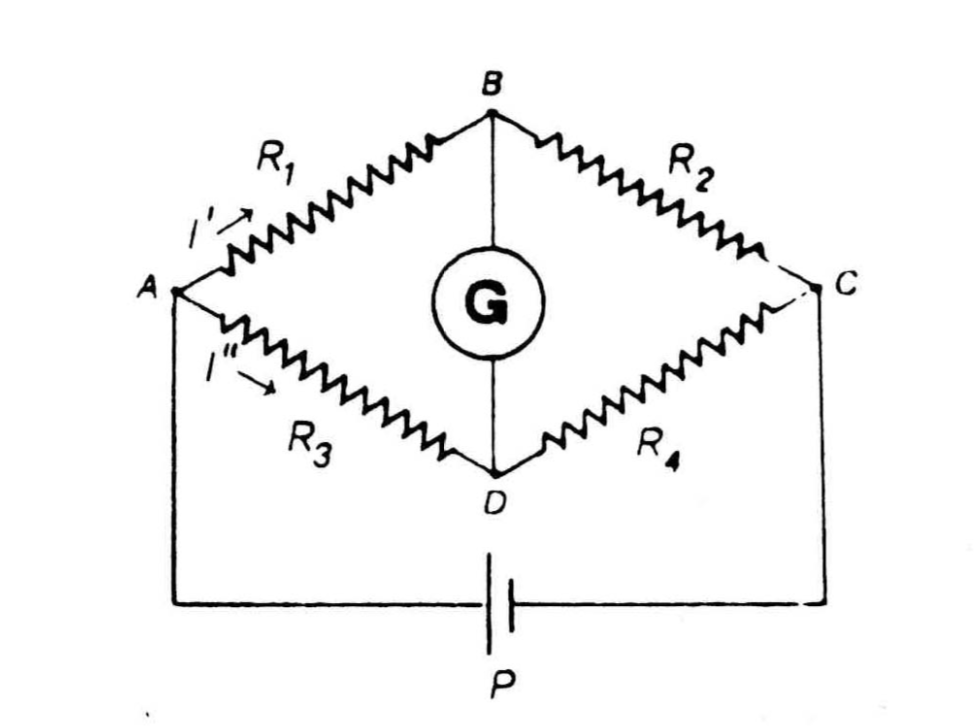
\includegraphics{pont}
	\caption{Esquema del pont de Wheatstone}
\end{figure}

\begin{figure}[h]
	\label{fig: <muntatge>}
	\centering
	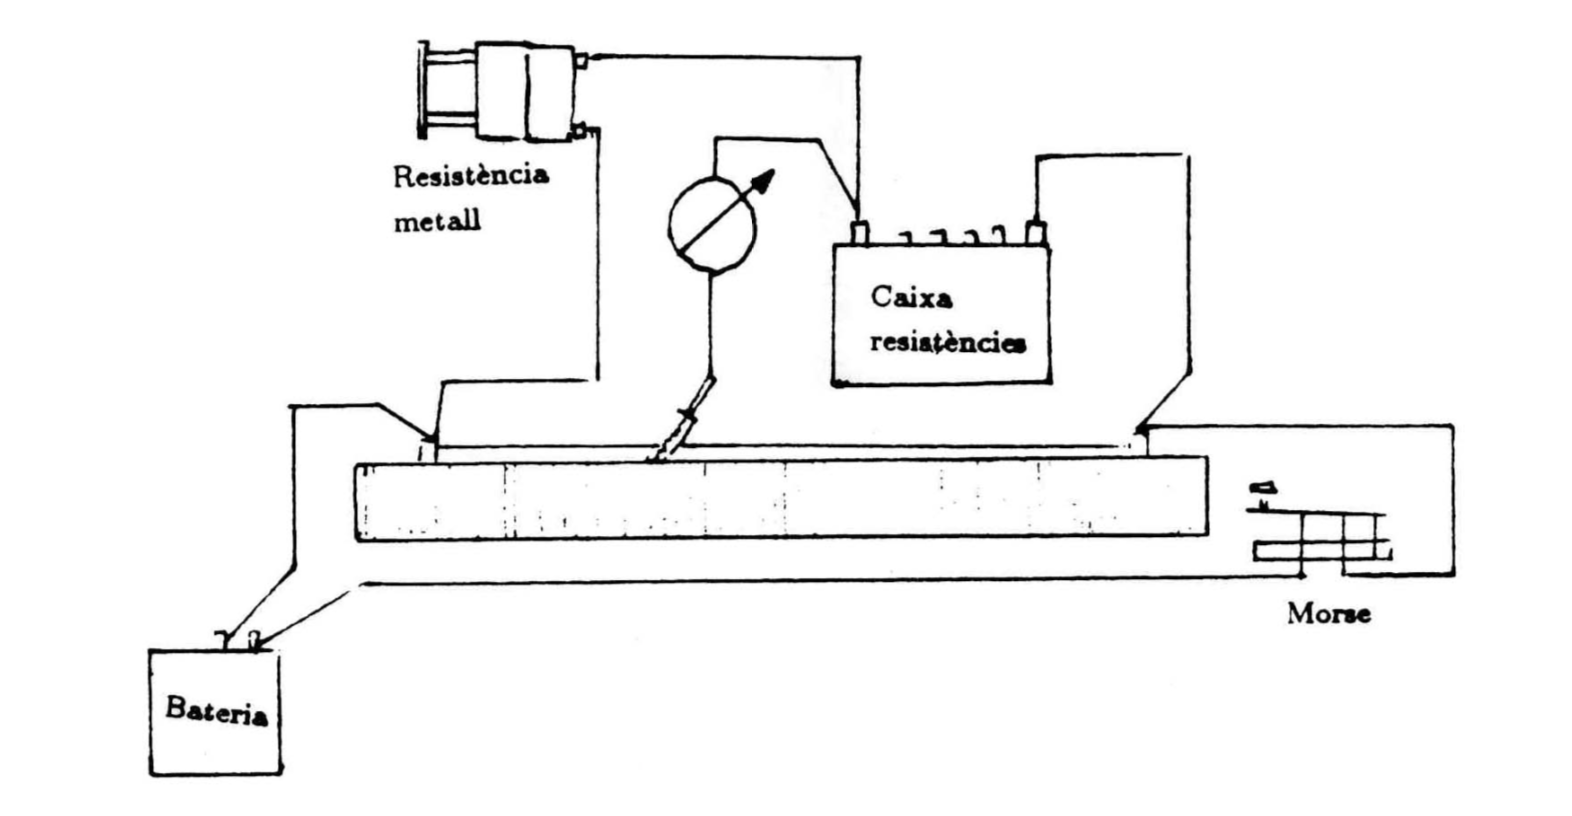
\includegraphics{muntatge}
	\caption{Esquema del muntatge experimental}
\end{figure}

\begin{equation}
\frac{R_1}{R_2}=\frac{R_3}{R_4}
\end{equation} 

En el pont de fil, dues de les resistències se substitueixen per un fil de longitud coneguda i un cursor que es pot moure per sobre. D'aquesta manera, existeix una relació directa entre el qupcient de les longituds i el quocient de les seves resistències. Usant una tercera resistència coneguda, $R_2$, la resistència incògnita, $R_1$ ve donada, quan el pont està balancejat, per

\begin{equation}\label{eq: <pont>}
R_1=\frac{x}{L-x}R_2
\end{equation}
on $x$ denota la longitud de fil a l'esquerra del cursor i $L$ la longitud total del fil. El muntatge experimental es pot veure en la \cref{fig: <muntatge>}. 

Les altes temperatures s'han obtingut introduint la resistència en un forn. S'ha deixat que aquesta prengués valors de fins a uns $\si{300}{\celsius}$ i s'han pres les mesures mentre es refredava a temperatura ambient. Les baixes temperatures s'han obtingut introduint la resistència en nitrogen líquid, i les mesures s'han pres mentre s'escalfava prop del nitrogen, per tal de reduir la velocitat a què ho feia i no perdre precisió.


\section{Resultats}

La \ref{tab: <results>} mostra la longitud $x$ a l'esquerra del fil a cada temperatura determinada, juntament amb la resistència del metall, usant \ref{eq: <pont>}. La longitud total del fil ha estat fixada en $L=\data{1.000}{0.001}{\meter}$ i la resistència externa en $R_1=\data{100}{1}{\ohm}$.

La regressió lineal amb les dades de la taula \cref{tab:<results>} es mostra en la Figura \ref{fig:<reg>}. El coeficient de correlació obtingut és de 0.997, el que demostra la linealitat de les dades en l'experiment considerat. S'han obtingut valors de $\data{0.359}{0.003}{\ohm\per\celsius}$ pel pendent i de $\data{106.9}{0.4}i{\ohm}$ per l'ordenada a l'origen. Relacionant aquests valors amb l'expressió \cref{eq: <regressio>} s'obté $R_0=\data{106.9}{0.4}{\ohm}$ i $\beta=\data{336}{3}e{-5}{\ohm\per\celsius}$.
%No se com posar exponencial amb incertesa al data. Ha de ser (336\pm3)\cdot10^{-5}

\section{Conclusions}
S'ha comprovat experimentalment la relació lineal entre la temperatura del metall usat i la seva resistència. El coeficient de correlació, de 0.997, demostra que existeix una relació com la descrita en l'expressió \ref{eq: <regressio>}. A més, s'han pogut determinar els paràmetres $\beta$ i $R_0$, amb valors de $\data{336}{3}e{-5}{\per\celsius}$ i $\data{106.9}{0.4}{\ohm}$ respectivament.
%Same here








\begin{table} \labelcref{tab: <results>}
	\centering
	\caption{Mesures experimentals de la resistència a diferents temperatures. El voltatge subministrat és aproximadament constat de $3.1\pm0.2\si{\volt}$}
	\begin{tabular}{|c|c|c|}
\textbf{Temperatura} $\data{}{1}{\celsius}$ & \textbf{Longitud $x$ } \data{}{0.001}{\meter} & \textbf{Resistència} \SI{\ohm} \\
265 & 0.664 & $\data{198}{9}{}$\\
260 & 0.668 & $\data{201}{9}{}$\\
255 & 0.665 & $\data{199}{9}{}$\\
250 & 0.664 & $\data{198}{9}{}$\\
245 & 0.663 & $\data{197}{9}{}$\\
240 & 0.661 & $\data{195}{9}{}$\\
235 & 0.659 & $\data{193}{9}{}$\\
230 & 0.657 & $\data{192}{9}{}$\\
225 & 0.655 & $\data{190}{9}{}$\\
220 & 0.654 & $\data{189}{9}{}$\\
210 & 0.646 & $\data{182}{8}{}$\\
200 & 0.643 & $\data{180}{8}{}$\\
190 & 0.637 & $\data{175}{8}{}$\\
180 & 0.630 & $\data{170}{8}{}$\\
170 & 0.627 & $\data{168}{7}{}$\\
160 & 0.622 & $\data{165}{7}{}$\\
155 & 0.620 & $\data{163}{7}{}$\\
150 & 0.616 & $\data{160}{7}{}$\\
145 & 0.613 & $\data{158}{7}{}$\\
140 & 0.610 & $\data{156}{7}{}$\\
135 & 0.608 & $\data{155}{7}{}$\\
130 & 0.605 & $\data{153}{7}{}$\\
125 & 0.603 & $\data{152}{7}{}$\\
120 & 0.600 & $\data{150}{6}{}$\\
115 & 0.597 & $\data{148}{6}{}$\\
110 & 0.593 & $\data{146}{6}{}$\\
105 & 0.585 & $\data{141}{6}{}$\\
23 & 0.520 & $\data{108}{5}{}$\\
-20 & 0.485 & $\data{94}{4}{}$\\
-25 & 0.484 & $\data{94}{4}{}$\\
-30 & 0.481 & $\data{93}{4}{}$\\
-35 & 0.478 & $\data{92}{4}{}$\\
-40 & 0.474 & $\data{90}{4}{}$\\
-45 & 0.470 & $\data{88}{4}{}$\\
-49 & 0.468 & $\data{88}{4}{}$\\
-55 & 0.464 & $\data{87}{4}{}$\\
-60 & 0.459 & $\data{85}{4}{}$\\
-65 & 0.457 & $\data{84}{4}{}$\\
-70 & 0.452 & $\data{82}{3}{}$\\
-75 & 0.447 & $\data{81}{3}{}$\\
-80 & 0.445 & $\data{80}{3}{}$\\
-85 & 0.441 & $\data{79}{3}{}$\\
-90 & 0.436 & $\data{77}{3}{}$\\
-95 & 0.431 & $\data{76}{3}{}$\\
-100 & 0.424 & $\data{74}{3}{}$\\
-105 & 0.417 & $\data{72}{3}{}$\\
-110 & 0.409 & $\data{69}{3}{}$\\
-115 & 0.398 & $\data{66}{3}{}$\\
-150 & 0.365 & $\data{57}{3}{}$\\
	\end{tabular}
\end{table}  
